\def\mySecNum{2.2}
\mySection{\mySecNum~Call options}
%-------------- start slide -------------------------------%{{{ 1
\begin{frame}[fragile,t]
\begin{center}
	Can one modify the forward contract so that\\
	the buyer can walk away from the deal at expiration?
\end{center}
\bigskip
\mySeparateLine
\bigskip

\begin{mydefinition}
	A \textcolor{magenta}{call option} is a contract where the buyer has the right to buy, but not the obligation to buy.
\end{mydefinition}
\bigskip

\end{frame}
%-------------- end slide -------------------------------%}}}
%-------------- start slide -------------------------------%{{{ 1
\begin{frame}[fragile,t]
	\begin{myexample}
		S\&R index: Buyers' perspective
		\begin{itemize}
			\item Today: call buyer acquires the right to pay \$1,020 in six months for the index, but is not obligated to do so
			\item In six months at contract expiration: \\
				if the spot price is \$1,100, call buyer’s payoff $=\$1,100-\$1,020=\$80$\\
				if the spot price is \$900, call buyer walks away, buyer’s payoff = \$0.
		\end{itemize}
	\end{myexample}

	\pause
	\bigskip
	\mySeparateLine
	\bigskip

	\begin{myexample}
		S\&R index: Sellers' perspective
		\begin{itemize}
			\item Today: call seller is obligated to sell the index for \$1,020 in six months, if asked to do so
			\item In six months at contract expiration: \\
				if the spot price is \$1,100, call seller’s payoff $=\$1,020-\$1,100=-\$80$\\
				if the spot price is \$900, call buyer walks away, seller’s payoff = \$0.
		\end{itemize}
	\end{myexample}
\end{frame}
%-------------- end slide -------------------------------%}}}
%-------------- start slide -------------------------------%{{{ 1
\begin{frame}[fragile]
\begin{center}
	\begin{minipage}{0.8\textwidth}
		\begin{itemize}
			\item[\textcolor{magenta}{Buyer}] preserves the upside potential, while at the same time eliminates the unpleasant
				downside.
				\bigskip

				\begin{align*}
					\text{However}
				\end{align*}
				\bigskip

			\item[\textcolor{cyan}{Seller}] has to be compensated by a initial premium for being at a disadvantage at
				expiration.
		\end{itemize}
	\end{minipage}
\end{center}
\end{frame}
%-------------- end slide -------------------------------%}}}
%-------------- start slide -------------------------------%{{{ 1
\begin{frame}[fragile,t]
	\begin{itemize}
		\item \textcolor{magenta}{Strike (or exercise) price}: the amount paid by the option buyer for the asset if he/she decides to exercise.
			\bigskip
		\item \textcolor{magenta}{Exercise}: the act of paying the strike price to buy the asset.
			\bigskip
		\item \textcolor{magenta}{Expiration}: the date by which the option must be exercised or become worthless.
			\bigskip
		\item \textcolor{magenta}{Exercise style}: specifies when the option can be exercised.
			\bigskip
			\begin{center}
				\renewcommand{\arraystretch}{1.2}
				\begin{tabular}{|c|c|}
					\hline
					Style                         & can be exercised              \\ \hline
					\textcolor{magenta}{European} & only at expiration date       \\
					\textcolor{magenta}{American} & at any time before expiration \\
					\textcolor{magenta}{Bermudan} & during specified periods      \\ \hline
				\end{tabular}

			\end{center}
	\end{itemize}
\end{frame}
%-------------- end slide -------------------------------%}}}
%-------------- start slide -------------------------------%{{{ 1
\begin{frame}[fragile,t]
	\begin{align*}
		\text{\textcolor{magenta}{Payoff} of purchased call} & = \max \left( 0, \text{spot price at expiration} - \text{strike price} \right) \\[1em]
		\text{\textcolor{cyan}{Profit} of purchased call}    & = \text{\textcolor{magenta}{payoff} of purchased call}                         \\
																												 & \quad -\text{future value of option premium}
	\end{align*}
	\bigskip
	\mySeparateLine
	\bigskip
	\begin{align*}
		\text{\textcolor{magenta}{Payoff} of written call} & = - \max \left( 0, \text{spot price at expiration} - \text{strike price} \right) \\[1em]
		\text{\textcolor{cyan}{Profit} of written call}    & = \text{\textcolor{magenta}{payoff} of written call}                             \\
                                                       & \quad + \text{future value of option premium}
	\end{align*}
\end{frame}
%-------------- end slide -------------------------------%}}}
%-------------- start slide -------------------------------%{{{ 1
\begin{frame}[fragile,t]
	\begin{myexample}
		 S\&R Index 6-month European call option
		 \begin{align*}
			 \text{Strike price}           & = \$1,000, \\
			 \text{Premium}                & = \$93.81, \\
			 \text{6-month risk-free rate} & = 2\%.
		 \end{align*}
		 Compute both payoff and profit of the \textcolor{alert}{purchased} call option if the index
		 value in six months $\textcolor{magenta}{\$1,100}$ (resp.  $\textcolor{cyan}{\$900}$).
	\end{myexample}
	\bigskip
	\pause
	\begin{mysol}\phantom{a}\\[1em]

	 \begin{minipage}{0.48\textwidth}
		\begin{center}
			If index value in six months = \textcolor{magenta}{\$1,100},
			\begin{align*}
				\text{Payoff} & = \max ( 0, \textcolor{magenta}{\$1,100} – \$1,000 ) \\
                      & = \$100                                              \\
				\text{Profit} & = \$100 – \$93.81 \times 1.02                        \\
                      & = \$4.32.
			\end{align*}
		\end{center}
	 \end{minipage}
	 \hfill \pause
	 \begin{minipage}{0.48\textwidth}
		\begin{center}
			If index value in six months = \textcolor{cyan}{\$900},
			\begin{align*}
				\text{Payoff} & = \max ( 0, \textcolor{cyan}{\$900} – \$1,000 ) \\
                      & = \$0                                           \\
				\text{Profit} & = \$0 – \$93.81 \times 1.02                     \\
                      & = – \$95.68.
			\end{align*}
		\end{center}
	 \end{minipage}

	 \myEnd
	\end{mysol}
\end{frame}
%-------------- end slide -------------------------------%}}}
%-------------- start slide -------------------------------%{{{ 1
\begin{frame}[fragile]
\begin{center}
	\includegraphics[scale=0.2]{figs/Figure-2-5.png}\hfill
	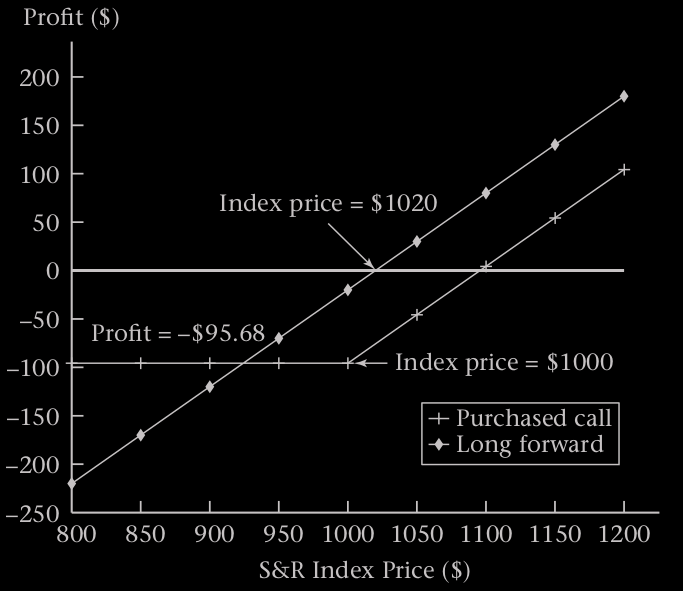
\includegraphics[scale=0.2]{figs/Figure-2-6.png}
\end{center}
\end{frame}
%-------------- end slide -------------------------------%}}}
%-------------- start slide -------------------------------%{{{ 1
\begin{frame}[fragile,t]
	\begin{myexample}
		 S\&R Index 6-month European call option
		 \begin{align*}
			 \text{Strike price}           & = \$1,000, \\
			 \text{Premium}                & = \$93.81, \\
			 \text{6-month risk-free rate} & = 2\%.
		 \end{align*}
		 Compute both payoff and profit of the \textcolor{alert}{written} call option if the index
		 value in six months $\textcolor{magenta}{\$1,100}$ (resp.  $\textcolor{cyan}{\$900}$).
	\end{myexample}
	\bigskip
	\pause
	\begin{mysol}\phantom{a}\\[1em]

	 \begin{minipage}{0.48\textwidth}
		\begin{center}
			If index value in six months = \textcolor{magenta}{\$1,100},
			\begin{align*}
				\text{Payoff} & = - \max ( 0, \textcolor{magenta}{\$1,100} – \$1,000 ) \\
                      & = - \$100                                              \\
				\text{Profit} & = - \$100 + \$93.81 \times 1.02                        \\
                      & = - \$4.32.
			\end{align*}
		\end{center}
	 \end{minipage}
	 \hfill \pause
	 \begin{minipage}{0.48\textwidth}
		\begin{center}
			If index value in six months = \textcolor{cyan}{\$900},
			\begin{align*}
				\text{Payoff} & = - \max ( 0, \textcolor{cyan}{\$900} – \$1,000 ) \\
                      & = \$0                                             \\
				\text{Profit} & = \$0 + \$93.81 \times 1.02                       \\
                      & = \$95.68.
			\end{align*}
		\end{center}
	 \end{minipage}

	 \myEnd
	\end{mysol}
\end{frame}
%-------------- end slide -------------------------------%}}}
%-------------- start slide -------------------------------%{{{ 1
\begin{frame}[fragile]
\begin{center}
	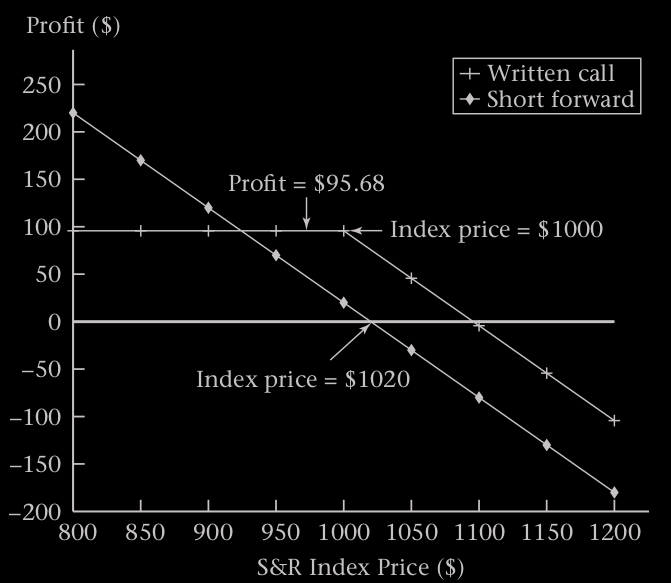
\includegraphics[scale=0.2]{figs/Figure-2-7.png}
\end{center}
\end{frame}
%-------------- end slide -------------------------------%}}}

